% ==============================================================================
% COVER / TITLE PAGE (Matches Official DIU FYDP Template)
% ==============================================================================
\begin{titlepage}
    \centering
    \setstretch{1.15}
    
    {\fontsize{18pt}{22pt}\selectfont \textbf{SMART LIBRARY MANAGEMENT SYSTEM}}\\[0.2cm]
    {\fontsize{14pt}{18pt}\selectfont \textbf{An Integrated Platform for Real-Time Seat Reservation, Physical Book Indexing, Digital Repository, and Automated Circulation}}\\[0.7cm]
    
    {\normalsize \textbf{By}}\\[0.25cm]
    {\normalsize \textbf{[Student 1 Full Name]}}\\[0.05cm]
    {\normalsize Student ID: [Student 1 ID]}\\[0.35cm]
    {\normalsize \textbf{[Student 2 Full Name]}}\\[0.05cm]
    {\normalsize Student ID: [Student 2 ID]}\\[0.65cm]
    
    {\normalsize \textbf{FINAL YEAR DESIGN PROJECT REPORT}}\\[0.25cm]
    {\small This Report Presented in Partial Fulfillment of the Requirements for}\\[0.05cm]
    {\small the \textbf{Degree of Bachelor of Science in Computer Science and}}\\[0.05cm]
    {\small \textbf{Engineering}}\\[0.65cm]
    
    {\normalsize \textbf{Supervised by}}\\[0.25cm]
    {\normalsize \textbf{[Supervisor Full Name]}}\\[0.05cm]
    {\normalsize \textbf{[Supervisor's Academic Designation]}}\\[0.05cm]
    {\small Department of Computer Science and Engineering}\\[0.05cm]
    {\small Daffodil International University}\\[0.55cm]
    
    {\normalsize \textbf{Co-Supervised by}}\\[0.25cm]
    {\normalsize \textbf{[Co-Supervisor Full Name]}}\\[0.05cm]
    {\normalsize \textbf{[Co-Supervisor's Academic Designation]}}\\[0.05cm]
    {\small Department of Computer Science and Engineering}\\[0.05cm]
    {\small Daffodil International University}\\[0.6cm]
    
    \vfill
    
    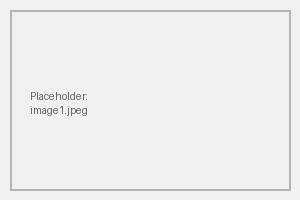
\includegraphics[width=1.35in]{./media/image1.jpeg}\\[0.35cm]
    
    {\normalsize \textbf{DAFFODIL INTERNATIONAL UNIVERSITY}}\\[0.1cm]
    {\normalsize \textbf{Dhaka, Bangladesh}}\\[0.05cm]
    {\small August 2026}
\end{titlepage}

\pagenumbering{roman}
\setcounter{page}{1}

% ==============================================================================
% APPROVAL PAGE
% ==============================================================================
\cleardoublepage
\section*{APPROVAL}
\addcontentsline{toc}{chapter}{Approval}

This Project titled ``\textbf{Smart Library Management System: An Integrated Platform for Real-Time Seat Reservation, Physical Book Indexing, Digital Repository, and Automated Circulation},'' submitted by \textbf{[Student 1 Name]} (ID: [Student 1 ID]) and \textbf{[Student 2 Name]} (ID: [Student 2 ID]) to the Department of Computer Science and Engineering, Daffodil International University, has been accepted as satisfactory for the partial fulfillment of the requirements for the degree of B.Sc. in Computer Science and Engineering and approved as to its style and contents.

\vspace{1cm}
\noindent\textbf{\underline{BOARD OF EXAMINERS}}

\vspace{0.8cm}
\begin{table}[H]
\centering
\begin{tabular}{p{8.5cm}r}
{[Board Chairman Name]} & \dots\dots\dots\dots\dots\dots\dots\dots\dots\dots \\
Board Chairman & Signature \\
Designation, Department of CSE, FSIT & \\
Daffodil International University & \\[0.8cm]

{[Internal Examiner 1 Name]} & \dots\dots\dots\dots\dots\dots\dots\dots\dots\dots \\
Internal Examiner 1 & Signature \\
Designation, Department of CSE, FSIT & \\
Daffodil International University & \\[0.8cm]

{[Internal Examiner 2 Name]} & \dots\dots\dots\dots\dots\dots\dots\dots\dots\dots \\
Internal Examiner 2 & Signature \\
Designation, Department of CSE, FSIT & \\
Daffodil International University & \\[0.8cm]

{[External Examiner Name]} & \dots\dots\dots\dots\dots\dots\dots\dots\dots\dots \\
External Examiner & Signature \\
Designation, Department of CSE, FSIT & \\
Daffodil International University & \\
\end{tabular}
\end{table}

% ==============================================================================
% DECLARATION PAGE
% ==============================================================================
\cleardoublepage
\section*{DECLARATION}
\addcontentsline{toc}{chapter}{Declaration}

We hereby declare that this project report titled \textbf{Smart Library Management System} has been carried out by us under the supervision of \textbf{[Supervisor Name]}, [Supervisor Designation], Department of Computer Science and Engineering, Daffodil International University. We further declare that neither this project nor any part thereof has been submitted elsewhere for the award of any academic degree, diploma, or certificate.

\vspace{1.5cm}
\begin{minipage}{0.48\textwidth}
\textbf{Supervised by:}\\[0.5cm]
\dots\dots\dots\dots\dots\dots\dots\dots\dots\dots\\
{\textbf{[Supervisor Name]}}\\[0.05cm]
{[Supervisor Designation]}\\[0.05cm]
Department of CSE, FSIT\\
Daffodil International University
\end{minipage}
\hfill
\begin{minipage}{0.48\textwidth}
\textbf{Co-Supervised by:}\\[0.5cm]
\dots\dots\dots\dots\dots\dots\dots\dots\dots\dots\\
{\textbf{[Co-Supervisor Name]}}\\[0.05cm]
{[Co-Supervisor Designation]}\\[0.05cm]
Department of CSE, FSIT\\
Daffodil International University
\end{minipage}

\vspace{2cm}
\noindent\textbf{Submitted by:}

\vspace{1cm}
\begin{minipage}{0.48\textwidth}
\dots\dots\dots\dots\dots\dots\dots\dots\dots\dots\\
{\textbf{[Student 1 Name]}}\\[0.05cm]
Student ID: [Student 1 ID] \\
Department of CSE, FSIT\\
Daffodil International University
\end{minipage}
\hfill
\begin{minipage}{0.48\textwidth}
\dots\dots\dots\dots\dots\dots\dots\dots\dots\dots\\
{\textbf{[Student 2 Name]}}\\[0.05cm]
Student ID: [Student 2 ID]\\
Department of CSE, FSIT\\
Daffodil International University
\end{minipage}

% ==============================================================================
% ACKNOWLEDGEMENTS
% ==============================================================================
\cleardoublepage
\section*{ACKNOWLEDGEMENTS}
\addcontentsline{toc}{chapter}{Acknowledgements}

We express our deepest gratitude to Almighty Allah for granting us the capability, perseverance, and determination to complete this Final Year Design Project (FYDP) successfully.

We express our sincere indebtedness and gratitude to our respected supervisor, \textbf{[Supervisor Name]}, for their continuous guidance, scholarly advice, and invaluable encouragement throughout every stage of this research and system implementation.

We also thank the Head of the Department of Computer Science and Engineering, faculty members, and library administration officers at Daffodil International University for providing institutional support, domain expertise, and technical facilities.

Finally, we express our profound appreciation to our parents and family members for their constant prayers, patience, and unconditional sacrifices.

% ==============================================================================
% ABSTRACT
% ==============================================================================
\cleardoublepage
\section*{ABSTRACT}
\addcontentsline{toc}{chapter}{Abstract}

Academic libraries in contemporary higher education institutions encounter severe operational bottlenecks stemming from manual seat management, physical book discovery latencies, uncoordinated resource lending, and disjointed digital media access. In large campus environments such as Daffodil International University, students frequently experience peak-hour seat congestion, double-booking disputes, and substantial delays locating physical volumes across multi-floor bookshelf arrays. To resolve these challenges, this thesis presents the \textbf{Smart Library Management System}, a unified, full-stack, cloud-ready software ecosystem that cohesively integrates real-time seat reservation, fine-grained physical book shelf indexing, digital PDF document repository access, and a staff-governed circulation lifecycle.

The system architecture utilizes a high-performance three-tier design combining a Next.js (React 19) responsive frontend, an Express.js (TypeScript) RESTful microservice backend, and a PostgreSQL database orchestrated through Prisma ORM. The platform incorporates four core innovations: (1) a concurrency-controlled seat reservation engine with dynamic slot allocation and cryptographically signed QR code check-in/check-out verification that automatically releases no-show seats; (2) a multi-dimensional physical indexing resolver that translates bibliographic search queries into exact spatial coordinates (Floor, Block, Rack, Shelf position, and Call number); (3) a secured digital repository allowing instant in-browser PDF preview and direct downloading for permitted electronic titles; and (4) an end-to-end borrowing and renewal management pipeline giving administrators and library staff comprehensive governance over checkouts, automated due-date extensions, fine computations, and real-time inventory tracking.

Experimental performance benchmarking validates that the proposed system eliminates double-booking occurrences (0\% conflict rate under concurrent stress testing), reduces seat acquisition time from a manual baseline of 14.5 minutes to under 25 seconds, and accelerates physical book discovery by 78.4\% through precise shelf coordinate guidance. API endpoints demonstrate average sub-45\,ms query latencies under sustained load. The project strictly adheres to BAETE Complex Engineering Problem (EP1--EP7), Knowledge Profile (K1--K8), and Complex Engineering Activity (EA1--EA5) accreditation standards.

\vspace{0.5cm}
\noindent\textbf{Keywords:} Smart Library Management, Seat Reservation System, Physical Book Indexing, QR Code Verification, Digital Repository, Library Circulation, Concurrency Control, Full-Stack Web Architecture.

% ==============================================================================
% TABLE OF CONTENTS, LIST OF FIGURES, LIST OF TABLES
% ==============================================================================
\cleardoublepage
\tableofcontents

\cleardoublepage
\listoffigures

\cleardoublepage
\listoftables
